\documentclass[../main.tex]{subfiles}

\begin{document}
\begin{multicols}{3}[
  Lo primer a efectuar antes de realizar ninguna operaión previa, es
  comprobar toda la instalación sobre la cual se va a efectuar el
  montaje de la red. En este caso el segundo piso del edificio del
  \textit{\acrfull{igg} de la \acrshort{unam}}. Nos piden lo siguiente:]

  \begin{itemize}
  \item El cableado de ochenta nodos de red con CAT 6a o superior.
  \item Dos \glspl{rack}.
  \item Cuatro \glspl{accp}
  \item \Glspl{PC} de categorías 6a o superiores de $24$ a $48$
    puertos.
  \item Correcto enrutamiento de lo IPs.
  \item Cableado de Fibra optica de \textit{doce hilos}, con cotización
    propia.
  \item Dos switch de cuarenta y ocho puertos $10G$ a un rango de
    $(390W, 450W)$.
    
  \end{itemize}
\end{multicols}

\subsection{Diseño Físico}\label{sec:disfis}

En la figura\ \ref{fig:dsp} Podemos apreciar
la ubicación de los racks de
telecomunicaciones y las áreas de trabajo.
También se nos proporciona un plano a detalle
donde se encuetran especificadas las
ubicaciones de las \glspl{roseta} y de
algunos \glspl{accp}, como un estimado de maquinas
a interconectar. En la siguiente sección (\ref{page:plano}) se muestra un
plano con el cableado ya estructurado.

\begin{figure}[H]
  \centering
  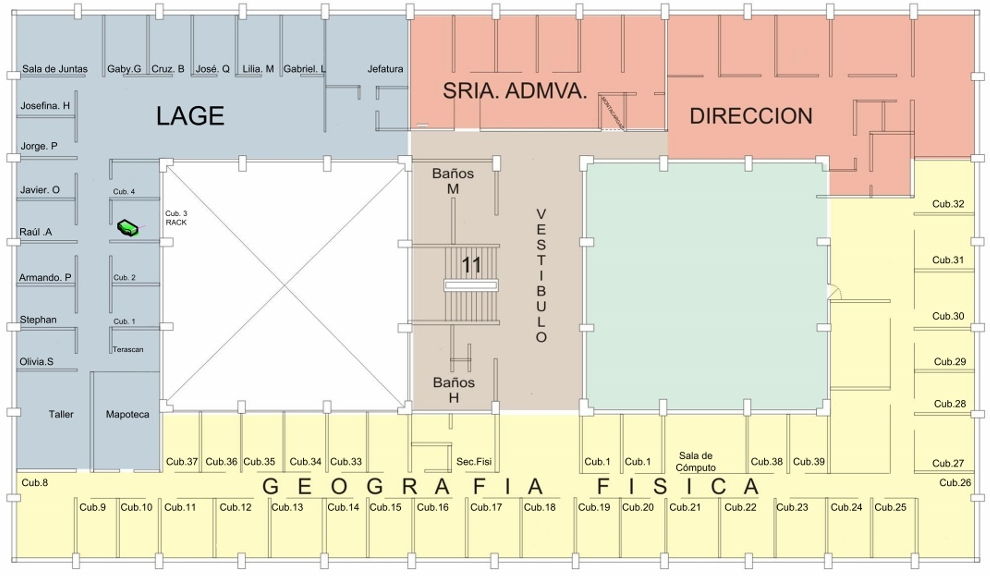
\includegraphics[width=1\textwidth]{2p.jpg}
  \caption{Distribución de la segunda planta}\label{fig:dsp}
\end{figure}



\end{document}
